\documentclass{scrreprt}
\usepackage[dutch]{babel}
\usepackage{graphicx}
\usepackage{etoolbox}
\usepackage{float}

%Remove newpage from chapter
\makeatletter
\patchcmd{\scr@startchapter}{\if@openright\cleardoublepage\else\clearpage\fi}{}{}{}
\makeatother
\DeclareGraphicsExtensions{.pdf,.png,.jpg}

\title{SOP6 Release Plan}
\author{Guus Hamm en Rick Rongen}
\date{\today}

\begin{document}
	\maketitle
	\tableofcontents
	\newpage
	\chapter{Verie Beheer Systeem}
	Als versiebeheer systeem wordt er git gebruikt in combinatie met GitHub en GerritHub. Met git kan er gemakkelijk verschillende branches gemaakt worden waardoor code onafhankelijk van elkaar beheert kan worden.
	GerritHub is een Gerrit applicatie die samen werkt met GitHub. Gerrit maakt van iedere commit een feature. Voordat deze commit in de origin branch komt te staan moet deze eerst gereviewd worden. 
	
	Door het gebruik van GitHub wordt er gebruik gemaakt van Open Source Software (OSS). Tevens bied GitHub de integratie met verschillende andere diensten en services zoals Continuous Integration of Code Review platforms. Gerrithub is tevens opensource maar zorgt er ook voor dat er transparantie is over hoe er geprogrammeerd wordt en wat de kwaliteits controle inhoud
	\chapter{Branches}
	\begin{figure}[H]
		\centering
		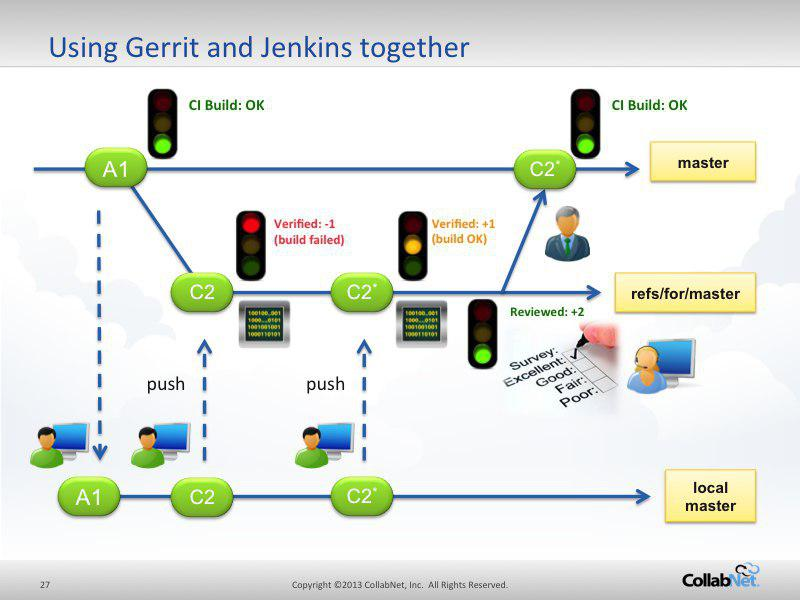
\includegraphics[width=\textwidth]{git-gerrit-jenkins}
		\caption{Branches}
		\label{img:branches}
	\end{figure}
	
	Gerrit maakt gebruik van verschillende soorten branches zoals te zien in figuur {\ref{img:branches}}. Een ontwikkelaar werkt op zijn lokale master branch. Zodra hij klaar is om zijn code naar jenkins te publishen kan hij een commit doen naar de refs/for/master branch. Deze branch bevat alle commit die normaal gezien de feauture commits zouden komen. Zodra deze refs/for/master branch is goedgekeurd wordt deze gepusht naar de daadwerkelijke master
	Er worden enkele verschillende branches gemaakt, zodat het product gestroomlijnd ontwikkeld kan worden. Dit zijn de branches: Release, Test en, Development. Er is geen feature branch omdat dit door Gerrit geregeld wordt, iedere commit is een feature.
	\chapter{Automatische Builds}
	Alle branches die op GitHub staan worden automatisch gebouwd door Jenkins. Dit is een automatisch systeem dat projecten kan bouwen, testen en uitbrengen. Hierdoor wordt er gecontroleerd of de code die online staat werkend is en ‘geen’ fouten bevat. Tevens zorgen deze tests ervoor dat er een build klaar staat van de code indien dit gewenst is. Deze build kan indien gewenst is direct gedeployed worden doormiddel van Continuous Delivery
	\chapter{Tests}
	Als het development team er zeker van is dat de code test waardig is, dan wordt deze op de test branch gezet. Hierna wordt dit door Jenkins gebouwd en kan het team deze versie testen. Als het testteam deze versie goed acht dan wordt deze versie doorgezet naar de Release branch en wordt er een nieuwe versie uitgebracht. Is het testteam van mening dat de kwaliteitsstandaarden niet behaald zijn dan kan dit in Gerrit worden aangegeven en zal de commit niet worden gemerged.
	\chapter{Hot Fix}
	Indien er een hot fix gemaakt moet worden dan zal dit door een administrator direct kunnen gebeuren buiten de code review om. Dit is echter een situatie die gereserveerd is voor noodgevallen. Normaliter zal dit alles via Gerrit gebeuren en zal deze ervoor zorgen dat hij in de release branch terecht komt.
\end{document}